\chapter{Introduction of PitchApp}
\chapterauthor{by Boglarka Lehoczki}

\section{The Value PitchApp Provides for Businesses}

PitchApp is intended to be a platform to help employees find the required organizational support to turn their ideas from inception to reality. The goal of our web-application is, thus, to facilitate the launching of new projects. By making project ideas of colleagues easier and faster visible to management, PitchApp encourages employees to contribute more actively to the success of the company at which they work. In this way, PitchApp helps to achieve higher degrees of intrapreneurship, which leads to business growth. Using our application will bring companies ahead of the game, in terms of innovation and
employee engagement, as well as make big firms more competitive and flexible, thus more
profitable. Hence, “fast innovators take leadership positions in their industries” \parencite{SH90}.

\section{Characteristics of PitchApp}

PitchApp is a dynamic, single-page web-application with database connection that we developed to enhance employee engagement and proactivity by connecting the employees’ ideas to even the highest levels of executives. Managers with budgets and resources for projects (i.e. potential future sponsors) can browse between different project ideas, which are posted by the employees. Distinct types of ideas are sorted into groups like HR, Procurement, R\&D etc., which facilitates searching among them. Then managers can offer their resources for the realization of a project idea, which they find valuable. Employees are also able to view the pitches posted by other colleagues in between their organization to avoid the sharing of redundant ideas. PitchApp is planned to be able to serve more large organizations at the same time and to be provided as a Software as a Service. PitchApp includes a user and session management system, which allows secure login and logout functionalities. It differentiates between public area, i.e. our landing page, and member area with two type of users, idea owners and idea sponsors.

\break

The table above shows how PitchApp fulfills the given project requirements.

\begin{center}
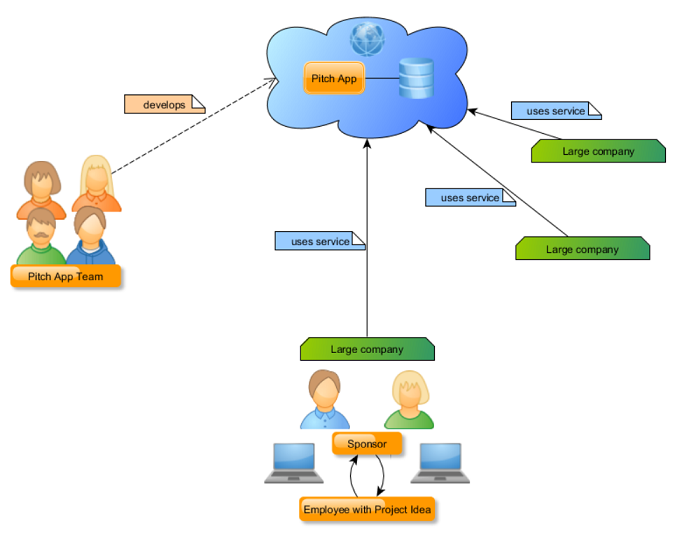
\includegraphics{pitchapp_saas.png}
\end{center}

The figure above presents the general characteristics of PitchApp.

\begin{table}[]
	\resizebox{\textwidth}{!}{%
		\begin{tabular}{@{}lll@{}}
			\toprule
			Requirement                                                                           & Status & Technology                \\ \midrule
			Log in / Log out (differentiation between public section and member area)             & done   & Okta                      \\
			User management                                                                       & done   & Okta                      \\
			Session management                                                                    & done   & Okta                      \\
			Application linked to a database                                                      & done   & PostgreSQL                \\
			Dynamic content                                                                       & done   & React single-page web-app \\
			Not high complexity, but challenging/latest technologies & done   & See above                 \\ \bottomrule
		\end{tabular}%
	}
\end{table}



\chapter{Architecture}
\chapterauthor{by Boglarka Lehoczki}

\section{Client-Server Architecture}

PitchApp implements a classic client-server architecture. More specifically, PitchApp is a web-application and has a 3-tier architecture. The three tiers are the user interface (UI), the application server and the database server. In such an architecture, the UI runs in a web-browser like Google Chrome or Mozilla Firefox. The UI communicates with the application server through HTTP requests and responses, as the application server also implements web-server functionalities. The application server itself acts as a client of the database server \parencite[p.~80]{MT17}. The interaction between these two servers can be based on different protocols or database connectivities, like JDBC for JAVA or ODBC for ABAP. In the case of PitchApp, this communication is solved by a Hasura GraphQL Engine, which auto-generates queries as part of the GraphQL schema from our Postgres schema model \parencite{Hasura}. The application server fetches the needed data from the database server, which returns it to the client in its reply. The process described above is shown by the following figure \parencite[p.~80]{MT17}.

\begin{center}
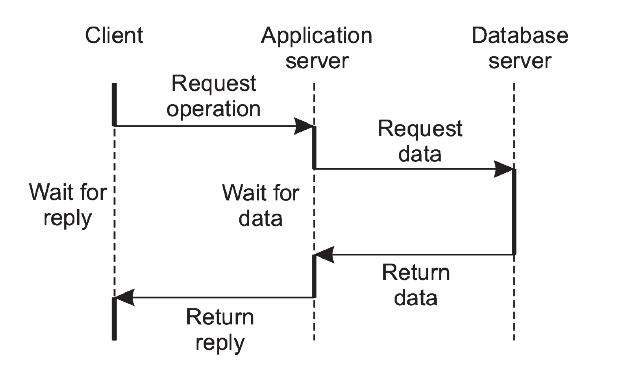
\includegraphics{3tiers_gen.png}
\end{center}

\break

The following figure gives a generalized example on how the tiers interact with each other when a user wants to see only those pitches, which were created by him or herself. This figure is based on another one from the book Distributed Systems \parencite[p.~61]{MT17}.

\begin{center}
	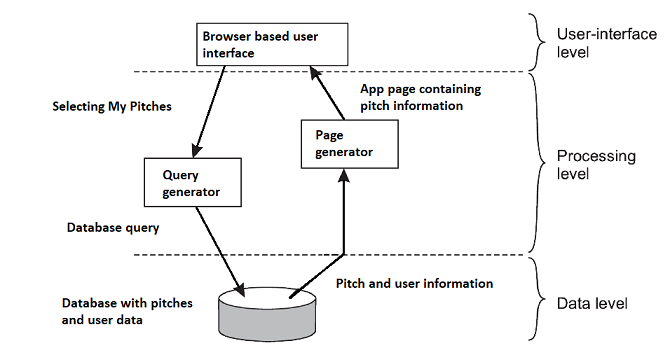
\includegraphics{3tiers_architecture.png}
\end{center}

Developing a web-application was a given requirement and it has several advantages. In comparison to a native application (with 2-tier architecture), the user do not have to install any additional application to its local machine, because the web-application runs in a browser. From this also follows, that if in the future we e.g. change the UI, users do not have to download updates onto their local machine. An other benefit of web-applications is that they are easier to scale and the different tiers can be scaled separately based on the use case. From the viewpoint of PitchApp this is particularly important, as our application has to be able to serve a large number of users from our customer companies.

\break

\section{Technologies used for each Tier of PitchApp's Architecture}

We selected state-of-the-art technologies to implement PitchApp. To develop a dynamic single-page web-application, React was used. With Reactstrap, we were able to create a responsive and neat-looking UI. Including an Okta modul to our web-application helped us to provide our users a secure authentication, user- and session management system. Our back-end is a Hasura GraphQL Engine which communicates easily with a PostgreSQL database. The following figure shows the architecture of PitchApp.

\begin{center}
	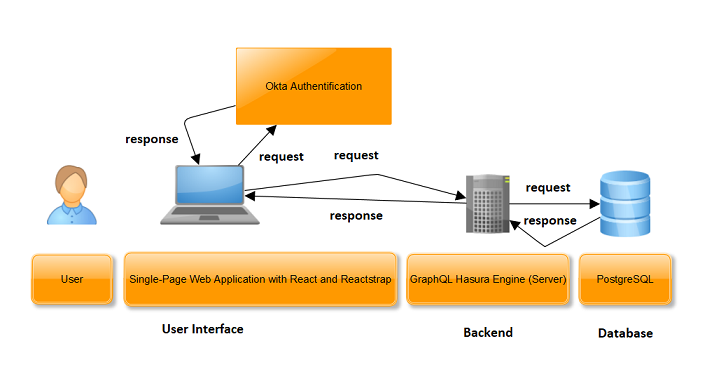
\includegraphics{pitchapp_architecture.png}
\end{center}


\chapter{Technologies used for Implementation}
\section{React and Reactstrap}
\chapterauthor{by Boglarka Lehoczki}

The client side of our web-application, PitchApp, was implemented by using React and Reactstrap, which is built on Bootstrap. The following figure presents how the relevant client side technologies are built on top of each other.

\begin{center}
	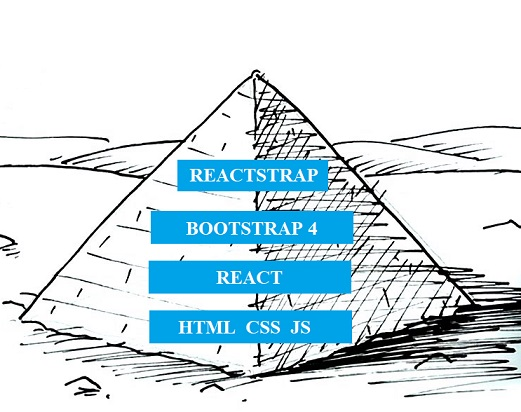
\includegraphics{pyramid.jpg}
\end{center}  

The basis of these web-technologies is the classical web-development trio of Hypertext Markup Language (HTML), Cascading Style Sheets (CSS) and JavaScript (JS). The .html, .css and .js files, which are executed to display the UI on the client side by the web-browser, are delivered by the web-server. HTML is used to describe the content of a web-page. CSS defines the design and layout of this content. JS is commonly used to implement further functionality and to build a dynamic web-page. JS is also called a scripting language, because it determines the way the content of the received web-page is parsed into the Document Object Model (DOM). In this way, the content of the received page can be manipulated. PitchApp was developed to fulfill the requirements of dynamic web-development and, through this, to achieve a higher level of user interactivity.

To achieve this, we used React, which is a JS library and helps to create web-based graphical UIs \parencite{React}. React works with JSX \parencite{JSX}, which can be described as a syntax extension for JS and combines characteristics of HTML and JS. As the basis of our web-application, a React App was created \parencite{Reactstrap}. The reasons, why we decided to implement PitchApp using React, are based on the general characteristics of React.

With this library, it is easy to develop interactive web-applications. React with JSX, just as JS, is used to access and manipulate the DOM of a web-page or web-application. It is done in the index.html file, where the root from <div id="root"></div> is replaced by all the content of PitchApp, which are to be found in the source folder (src directory) and collected into one component <App/>. In the index.js file, the React DOM is mapped to the root with the following code: ReactDOM.render(<App />, document.getElementById('root'));.

React is declarative and component-based. This means, that the presented UI elements are programmed as a component and can be used and rendered when needed to the UI. The following example shows code snippets from Home.js, which is the landing page of PitchApp and HomeJumbotron.js, which is a jumbotron component of PitchApp displayed on the publicly available landing page.

\begin{center}
	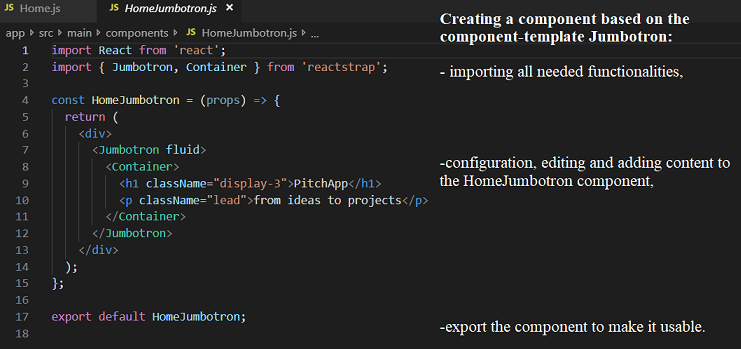
\includegraphics{home_jumbotron.png}
\end{center} 

\begin{center}
	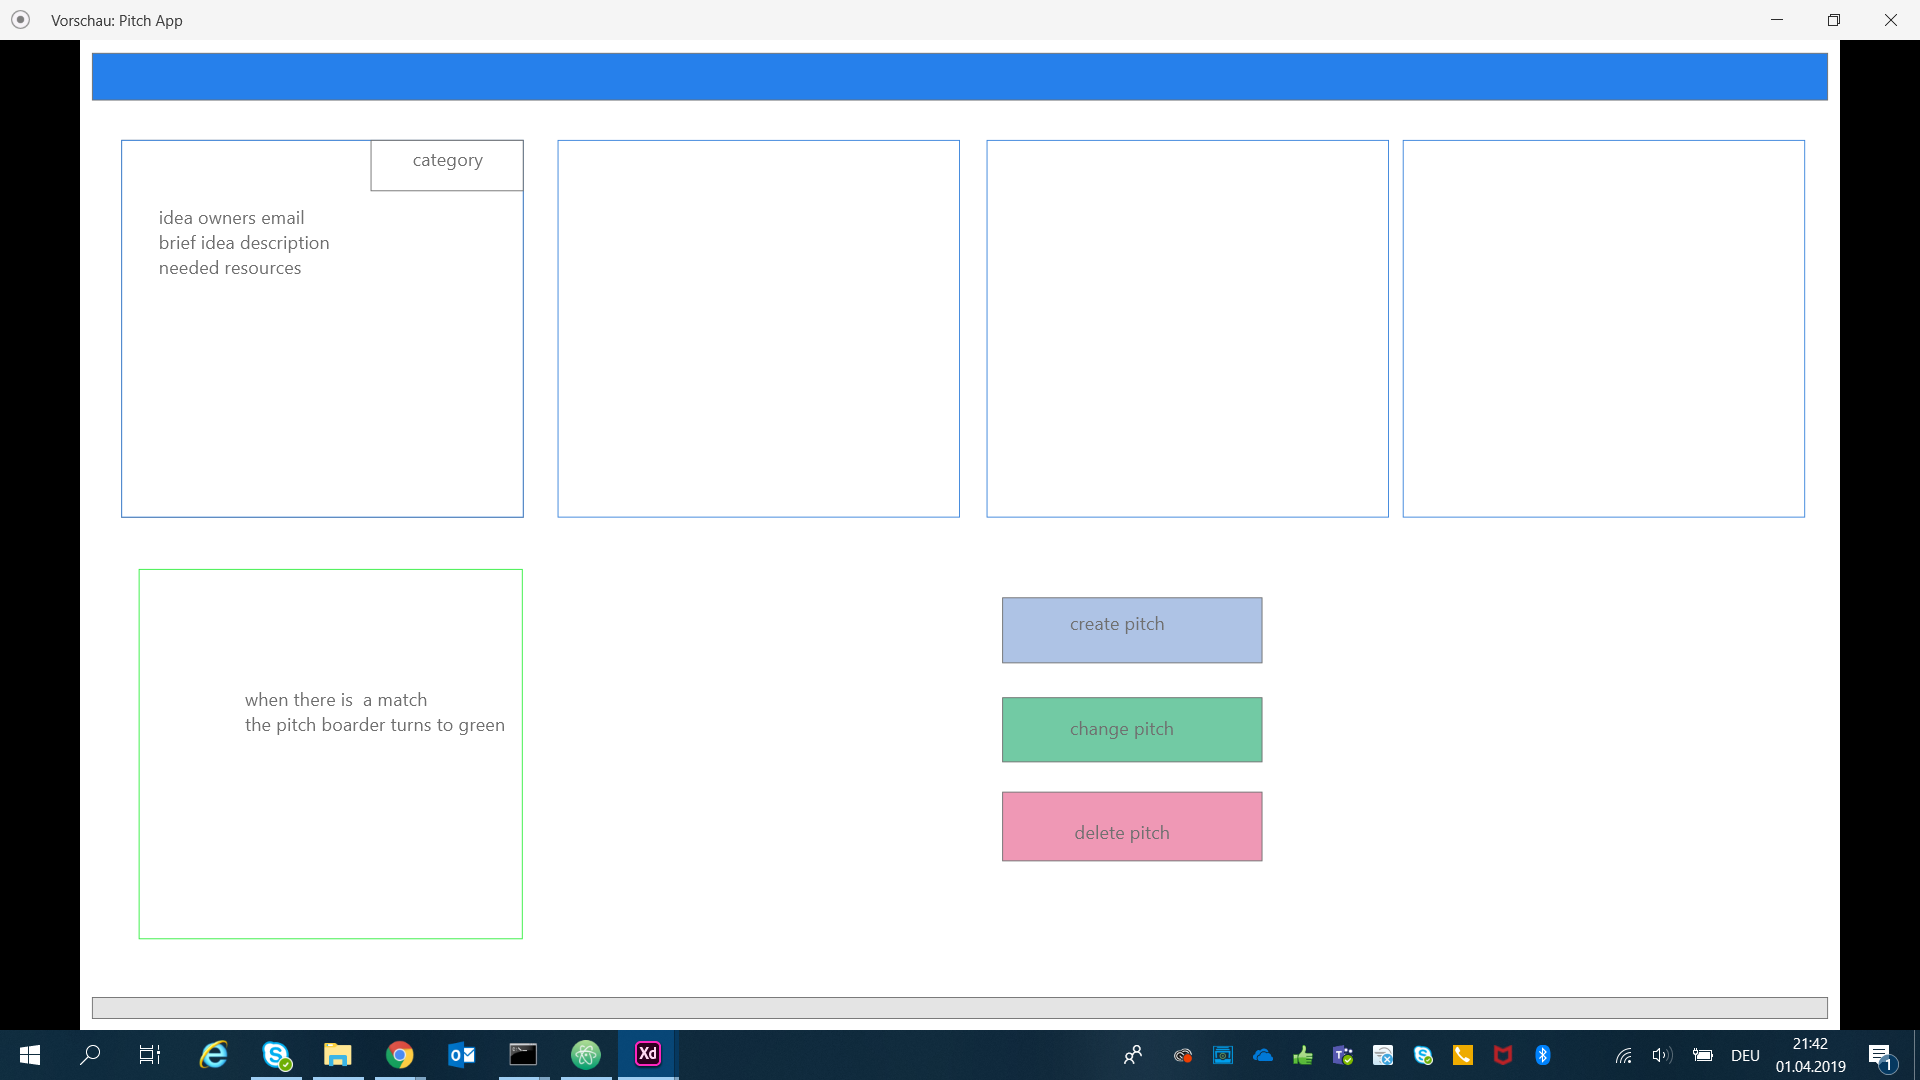
\includegraphics{home.png}
\end{center} 

Instead of designing the appearance of our own UI elements, which would cost us high effort, we were enabled to use already designed component-templates from Reactstrap \parencite{Reactstrap_comp}, combine them and - as a result - get a complex, yet neat looking UI design. In this way, we only had to decide how we combine these component-templates to create our own Reactstrap components. Our goal was to represent the users an intuitive UI. Furthermore, PitchApp was developed to be an "idea pool", where ideas of users must be very straightforward to collect and display. We also needed a simple way to represent states of Pitches, i.e. if a Match occurred to a Pitch. A Match means that an idea sponsor found that a posted idea (Pitch) is worth to be realized. This problem is also solved component-based. Each component manages states internally, which facilitated the handling of different states of UI elements. A render() method is implemented in each of the React components. This method takes input data and returns what to display. Render() can access input data by the attribute named "this.props". Internal state of a component can be accessed similarly with "this.state". Our goal was to build a convenient UI, where employees share their ideas happily and managers can smoothly brows between these. We used - inter alia - the Reactstrap components Badge to indicate a Match, Buttons to enable user interaction by clicking to navigate inside PitchApp, Jumbotron for an attractive landing page design, Media to include our logo and Modals to display additional information to the users.

React is compatible with Node, which we have also used on the server side for our back-end implementation. In other words, Node.js is a runtime environment for JS, with which React code can also be compiled.

An other advantage of React, that it is secure. By programming in JSX, it is safe to embed user inputs. React DOM escapes values coded in JSX before rendering them and all input is converted to string before rendering \parencite{JSX}. In this way, protection against injection attacks, especially against cross-site-scripting, is provided.

Additionally, Bootstrap \parencite{Bootstrap} should be mentioned, because Reactstrap component-templates are based on Bootstrap 4. Using the Bootstrap 4 layout grid system (more information can be found on \parencite{Bootstrap_grid}) facilitated the creation of a responsive UI, which was an explicit requirement for PitchApp. For this reason, Pitch App follows the principles of responsive web-design, which means that our web-application can be used on various sizes of screens including mobile phones and tablets. The UI components of PitchApp are able to automatically resize and move to display a nice-looking view on all kind of devices or window-sizes.

The following figures show how a full window-size version and a small window-size version of PitchApp's UI look with the reorganized UI elements.

\begin{center}
	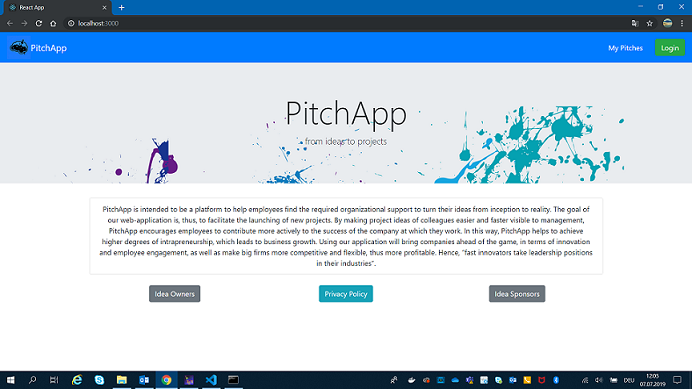
\includegraphics{pitchapp_big.png}
\end{center} 

\begin{center}
	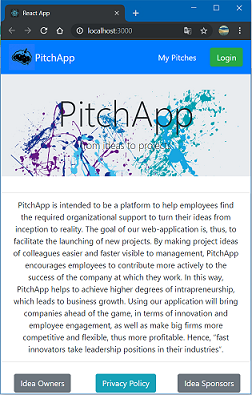
\includegraphics{pitchapp_small.png}
\end{center} 

During the design phase of PitchApp, our team decided to construct PitchApp to be a single-page web-application to enhance user experience. A single-page web-application intends to mimic the advantage of a desktop application and to avoid the unnecessary interruption of the user by saving navigation effort and time. The underlying idea is that, instead of loading whole page content repeatedly to the screen, only the changes are rendered. For example, PitchApp shows all the pitches on its Dashboard and, when a user filters pitches by category, PitchApp does not redirect to an other page, but still displays the selected pitches on its Dashboard. React adopts the principles of developing single-page applications, which was another argument for using React to the development of PitchApp. We used React routing components, like Router, Route, Redirect and History for managing session history, to achieve single-page rendering in PitchApp's App.js. Detailed explanation of different routing components with React can be found on reacttraining.com \parencite{React_router}.

To sum up, we can state that PitchApp was developed by using React and Reactstrap to be:

\begin{itemize}
	\item interactive,
	\item intuitive,
	\item secure,
	\item compatible,
	\item combinable,
	\item attractive,
	\item simple,
	\item single-page,
	\item responsive and
	\item dynamic.
\end{itemize}

\section{Okta Authentication}
\chapterauthor{by Ethan Kelly}

The User Management, Authentication \& Authorization along with Session Management for PitchApp is handled using the Okta Identity and Access Management Platform. Okta was chosen on the basis that it is fully OAuth 2.0 compliant, fully scalable and architected for zero downtime. Okta also offer many tools and services to help us with compliance and data security which we will discuss in the coming sections.

\subsection{Identity and Access Management (IAM)}

Identity and Access Management (IAM) are the framework of policies and technologies that ensure the proper people in an enterprise have the appropriate access to technology resources. Identity management can involve 4 basic functions:

\begin{itemize}
	\item Pure Identity – In all practical models of digital identity, a given identity object consists of a finite set of properties (attribute values). These properties record information about the object. A "pure identity" model is strictly not concerned with the external semantics of these properties.
	\item User Access - User access enables users to assume a specific digital identity across applications, which enables access controls to be assigned and evaluated against this identity. Access management is normally the motivation for identity management.
	\item Services - Many products require identity management to properly provide their services as they often require access to extensive information about a user which is subject to privacy and/or confidentiality requirements.
	\item Identity Federation - Identity federation comprises one or more systems that federate user access and allow users to log in based on authenticating against one of the systems participating in the federation. This trust between several systems is often known as "Circle of Trust". When a user needs to access some service controlled by SP, he/she first authenticates against the IdP and if successful an assertion is sent to the Service Provider.
\end{itemize}

Along with the capability to create, modify and delete identity data, Identity Management systems control data access and use across systems. To do this the system should have the following capabilities:

\begin{itemize}
	\item Authentication – Is the verification of if a user is who they say they are
	\item Authorization – Means managing what operations a user can execute.
	\item Roles – Roles are groups of operations or other roles which relate to a user’s job/tasks.
	\item Delegation – Delegation is the ability to allow another user to carry out tasks on your behalf.
	\item Interchange – The system needs a way of exchanging identity information across systems. The SAML and OpenID Connect protocols are common examples of such methods.
\end{itemize}

\subsection{The Shared Security Responsibility Model}

Okta makes use of the shared security responsibility model, a model used by many cloud providers including Amazon AWS and Microsoft Azure. This model specifies the distinct responsibilities of us (the customer) and the cloud provider.

\textbf{Okta's Responsibility}

Okta is responsible for the security of the Okta Identity Cloud Platform and its underlying infrastructure. They also provide features to allow us to fulfill our responsibilities.

\textbf{Our Responsibility}

We are responsible for securing our application using the features that Okta offer. This includes granting the correct permissions to users, protecting the right areas of the application and its data to ensure only authorized users see this information.

\begin{center}
	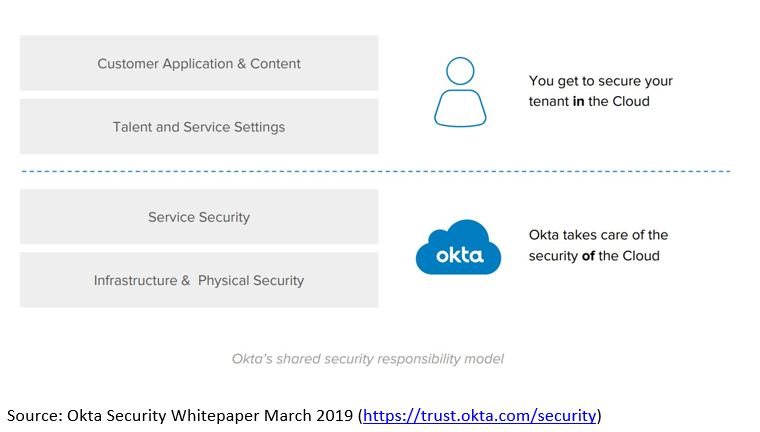
\includegraphics{okta1.png}
\end{center}

\subsection{Authentication and Authorization}

\textbf{Authentication}

As mentioned earlier, authentication is the process to verify if a user is who they say they are. Okta handles authentication for PitchApp. When users click Login within PitchApp they are forwarded to our Okta login page. Here users are given the opportunity to enter their login details. When users are registered by their company, they receive an email to confirm their email address. After successful registration the user is returned to PitchApp. When Okta redirects the user back to PitchApp it provides an authorization code and a user context that can be used within the app.

\textbf{Authorization}

PitchApp will then use this authorization code along with the required scope to request an access token from Okta. If the user is authorized to use such a scope an access token is returned. This token is then used when the user tries to use a restricted functionality of PitchApp, for example, sponsoring a Pitch. These tokens are also used by PitchApp to ensure users are only able to see information or Pitches, which they are authorized to see.
Okta works with Role-based Access Control which allows us to provide our customers with an even more personalized experience, while maintaining the upmost level of data security. Okta is also fully OAuth 2.0 compliant, this allows us to easily make use of the Role-based Access Controls, revoke access, and manage the token lifestyle. OAuth 2.0 is the industry standard protocol for authorization. It allows a user to gain limited access to a HTTP service.

\begin{center}
	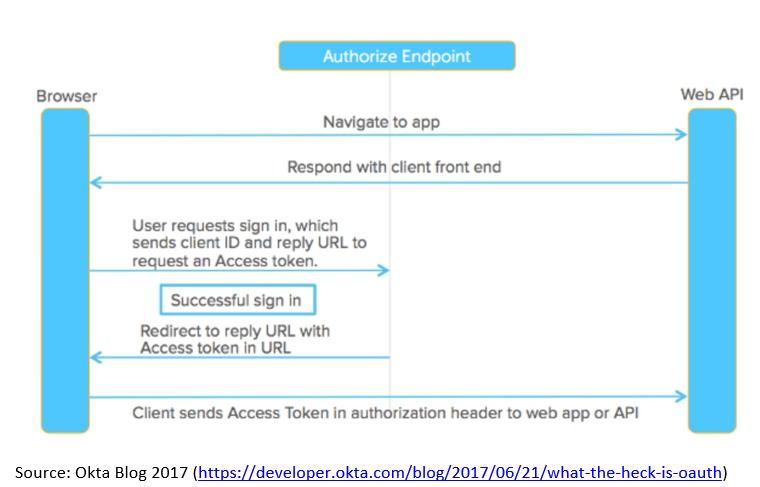
\includegraphics{okta2.png}
\end{center}

\subsection{Session Management}

A web session is a series of HTTP requests and responses created by the same user and session management is the set of rules that governs interactions between websites and its users. Sessions are established at a certain point in time, usually at the time of authentication, and torn down usually at the time of logout or after a timeout. There are 2 forms of session management, cookie-based and URL-rewriting.
Okta uses a cookie-based authentication mechanism to maintain a user's authentication session across web requests. Session cookies have an expiration configurable by an administrator for the organization and are valid until the cookie expires or the user closes the session (logout) or browser application. A session token is returned after successful authentication which can be later exchanged for a session cookie. Encrypted connections are used for all communications with Okta.

\pagebreak

\section{GraphQL Hasura Engine as Server}

\chapterauthor{by Csaba Kegyes}

\textbf{GraphQL}

GraphQL is a query language that provides a technology for having a unified interface for a variety of database systems. For example, it will allow a user to use SQL and MongoDB databases, together. A GraphQL server is usable by common REST calls.
 
One of the reasons why we decided to use GraphQLis that it integrates quite well to React through Apollo. This could be due to the fact that both technologies are developed by Facebook. This integration meant that we did not need to develop our own API for a database, defining both the end-points and the queries themselves. For example, by using MongoDB we would have had to host the database itself and a server that is running a MongoDB driver. Accessing the database directly through REST calls is possible but highly insecure.

The GraphQL client in our React application also provides us with more ease of use for development. For instance, the GraphQL client can redo queries on select intervals or when it detects changes; this functionality is built into the client natively, so we didn’t have to use sleep methods or loops for this purpose.

One downside of using GraphQL is that defining the queries is a long process that cannot be changed during run-time. Besides the queries, type definitions, resolvers also have to be defined. This means that a query doesn’t have to be edited in one file in a centralized manner but in at least three.

\textbf{HasuraGraphQL Engine}

After making our prototype GraphQL server we discovered some of the shortcomings of the technology. Making changes to our schema would require us to redo our GraphQL server as well. And also we could run into some trouble when trying to put this server into a Docker container. We elected to use HasuraGraphQL Engine to try to correct some of these shortcomings.
 
One of the main positives of Hasura is the ability to generate queries and mutations on the fly. When a new table or column is created in the database connected to Hasura, it automatically generates the methods for CRUD operations. This enabled us to run the server and experiment with the data freely.
Hasura also provides us with Docker files and docker images that we could use for deployment later, whether on a serverless environment like Heroku or on our own Virtual Private Server. 


\section{PostgreSQL Database}

\chapterauthor{by Csaba Kegyes}

PostgreSQL is an open source object-relational database which highlights extensibility and serves a variety of technical standards. We chose to use Postgres because its integration with the HasuraGraphQL engine. Hasura uses it by default and because its availability as an official docker image we can also run it in a containerized way.
 
We also found that the way relational databases represent data was easier to work for us than document-based ones, for example in MongoDB. This could be because of our familiarity with SQL through our courses at DHBW Mannheim.

Our pitch table in our Postgres database is constructed the following way:

\begin{center}
	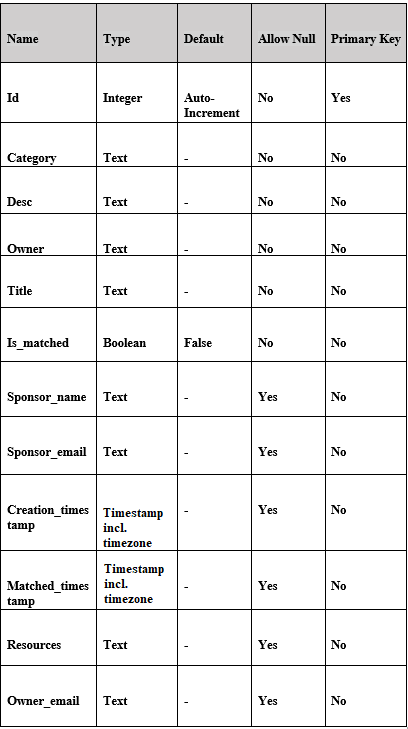
\includegraphics{db_table.png}
\end{center}

\section{Docker}

\chapterauthor{by Csaba Kegyes}

Docker is an open source tool that uses containers in order to assist both developers and system administrators to create, implement and run applications. Through the containers the application can be shipped in one package along with all its components such as code, libraries, tools etc.

We decided to use Docker in order to have a clearer separation of reusable components, similar to a micro-service oriented design. With Docker we can get some components that are provided by the developers themselves, like in the case of Hasura and Postgres but we can also make our own one for the React front-end application.

With this clear separation we could have much more flexibility when deploying for ourselves or for a potential customer. The components, the front-end, HasuraGraphQL engine, Postgres database, do not have to be on the same server, or hosted on a service that is offered by one provider. For example, the instance that we have provided already uses Heroku for hosting the database and the GraphQL server, while we used Firebase, which supports single-page web applications, to host our front-end.

In a real-life scenario, containerizing our application would be important because it also allows us to run the applications with popular orchestrators, such as docker swarm or Kubernetes. Providing the safety and automation offered by these technologies is essential for selling a web-service.

For our application we have three containers. One of them is the HasuraGraphQL engine. The image is provided by the developers. One of the other containers is the Postgres database. It is also an official image that can be found on docker-hub. Our third container is the front-end one. In order to build this we first had to run build on our React project that was created using the utility create-react-app. The build folder that was created by this script is included in the image, which is then served by Nginx. Nginx also needed a custom configuration files to handle a single-page web application.

These three containers are deployed using a docker-compose file that includes configuration for the ports, volumes and other characteristics so that the three components can work together.

We have put PitchApp from development mode to a productive mode with Docker by running the following command:

npm run build

This creates a build folder in the same directory that can be served by the npm build serve method or by using other servers, such as Nginx.

After the build process was done the PitchApp could be put into a container. There is already a Docker file that specifies how this should be done using a base Nginx image. So we run the following command in the command line:

docker build -t "NAME OF IMAGE" .

The name of the image in our case is pitch-docker.

This image can be used separately, as well as the developer and production builds.


\chapter{Final Results}

\chapterauthor{by Stella Kamakari}

\textbf{Public Section}

The public section of PitchApp is comprised of a single web page that guests visit when they want to use the application. This web page presents the main idea behind PitchApp, information for idea owners and idea sponsors, as well as our privacy policy about how PitchApp protects the ownership of ideas. Finally, it includes a button to sign in with Okta or the user can click on the My Pitches button to do the same. Once the user logs in with his or her email address as user name and password, he/she can access the rest of the functionality offered by PitchApp, depending on whether the user is an idea owner or a sponsor.

\textbf{Registered User Area}

The user area for both the idea owner and the idea sponsor have been implemented as planned. The main features for an idea owner are pitch creation, pitch deletion, and showing sponsor information in the event of a match.
Pitch creation is handled by an appropriate form that enables the user to enter a title for the Pitch, the general area that is pertinent to the Pitch (e.g. HR or Procurement), the Pitch’s description, as well as resources that are required for its completion.
Pitch deletion is as easy as clicking on a button and can be performed only by the user who created the pitch. With this, we ensured that none else can delete a pitch except the idea owner him/herself.
In case of a match, the idea owner can also see the information of the sponsor that matched it. In particular, it shows the name and e-mail address of the sponsor as well as the exact time when the match took place. After that, it is up to the pitch creator to contact the sponsor that matched the pitch.

The main feature of idea sponsors is to view pitches and specific information about them, as well as offer a match to a pitch. When sponsors log in, they view a list of available pitches if these have been previously created by colleagues.
A sponsor can view the information of a pitch that its owner registered when the pitch was created. A sponsor can then match a pitch, which is as simple as clicking on a button. The pitch creator then receives the information of the sponsor as described above.
Finally, sponsors can filter pitches based on their general area, so they can focus on the pitches they are more interested in. If they want to return to browse among all pitches again, they can click on Show All Pitches in the Search Pitches by Area dropdown or on the logo on the top left.

\textbf{User Management}

In PitchApp, user management is done by using services offered by the Okta Identity and Access Management Platform. These services include:

\begin{itemize}
	\item User account creation using Okta registration form, with features such as email address confirmation,
	\item login to user account and logout,
	\item role-based access control, which allows the implementation of different user types, i.e. idea owner, idea sponsor and
	\item cookie-based authentication for session management.
\end{itemize}

It is worth to mention that all network communication with Okta’s services uses encryption.

Users from companies receive an email from Okta, where they follow the steps of registration by e.g. setting their password. These registration emails are generated on demand of the companies by our team. In this way, companies can define how many and exactly for which co-workers they want to provide access to the application.

To demonstrate the full capabilities of PitchApp and test its functionalities, we created a third user type - a super user - which has the rights of both sponsors and idea owners. This kind of user was provided in order to evaluate and note PitchApp.

\textbf{Linked to a Database}

The functionality of PitchApp is based on database access. The database chosen for PitchApp was PostgreSQL, an open source object-relational database. The motivation for choosing PostgreSQL includes the following reasons.
First, PostgreSQL integrates with the Hasura GraphQL engine, another technology that simplifies database access. Second, PostgreSQL made it possible to use docker images easier as well, which enabled for simpler deployment of PitchApp. Finally, PostgreSQL was selected because our development team was already familiar with relational databases, as opposed to document-based databases such as MongoDB.

\textbf{Dynamic Content}

PitchApp is a dynamic application. Information is updated in various areas of the application appropriately. The users, be it idea owners or idea sponsors, view updated information at all times.
In particular, when an idea owner submits a pitch, it becomes viewable to all other owners and idea sponsors. Furthermore, any sponsor has the possibility to offer a match to a pitch. When that happens, the information of the sponsor as well as when the match happened appear on that pitch (which can be viewed by the creator and the other registered users).

\chapter{User Manual - Running PitchApp}

\chapterauthor{by Stella Kamakari}

\section{Way 1 - Accessing the Deployed Version}

We have a working site that can be reached at: https://pitchapp-9f7e5.firebaseapp.com

Also, an instance of the database interface can be reached at https://db-for-pitch.herokuapp.com/console

\section{Way 2 - Running the Local Productive Build}

For PitchApp, the optimal way to run the whole application is through Docker. We have provided a docker-compose file that takes all of the images that are needed and runs them on the proper ports. As it was discussed before in the respective chapters the images that are taken for HasuraGraphQL Engine and Postgres are official ones. However, the one for PitchApp is our own that was uploaded to DockerHub with the account of Csaba Kegyes.
 
Using the command line the following command should be ran from the folder where our docker-compose.yaml file is located:

docker-compose up

This command will automatically download the images and start the application. The application can be reached at localhost:8000. Hasura database interface is accessible at localhost:8080. After accessing the database interface, one should navigate to the "DATA" button on the top in the grey navigation bar. When running PitchApp this way, the database table - that we have described in Chapter 3.4 about PostgreSQL and have also included here for convenience, has to be created for the application to work. So the next step is to click on the yellow button "Create Table" by leaving the Schema Dropdown at "public". The created table has to have the name "pitch" and contain the following columns with parameters:

\begin{center}
	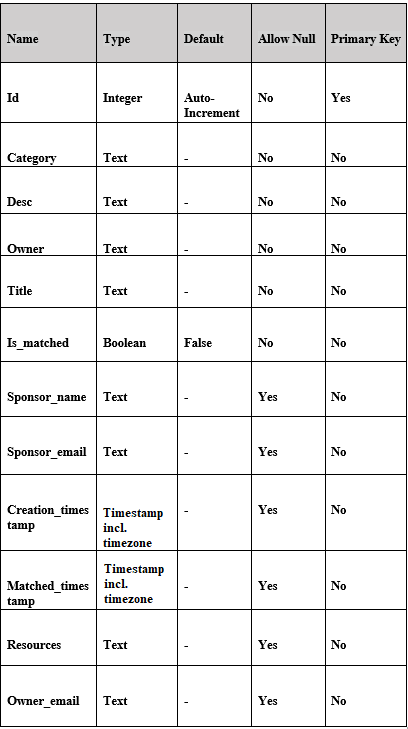
\includegraphics{db_table.png}
\end{center}

After this table is created, one can add the data regarding a pitch to it by the button "Insert row". The rows of this table can be also manipulated from the UI of PitchApp by adding a pitch or deleting a pitch. One can only delete a pitch, which was added by him/herself before.


\section{Way 3 - Running the Development Mode}

In order to run PitchApp in development mode, open up a terminal and navigate to the 'app' folder in our repository. First the dependencies should be installed. This can be done by the following command:

npm install

Npm stands for node package manager.

After this is done, the application can be run in developer mode by entering the command:

npm start

It will open PitchApp on localhost:3000. This version does not have a database connection.

In order to connect the development version of PitchApp with the database, a second terminal window should be opened and the database should be started manually with the command:

docker-compose up

\section{Implemented Features}

\textbf{Public Section}

Through the public section, a user can perform the following actions:

\begin{itemize}

\item To view information about idea owners, the user must press the button “Idea Owners”.
\item Likewise, users can see information about idea sponsors by pressing the button “Idea Sponsors”.
\item The privacy policy of PitchApp is accessible by clicking on the corresponding button.
\item To login, the user can click on the “Login” button. The same thing happens when the user clicks on the button “My Pitches” as well.

\end{itemize}

\textbf{Login Section}

The user can sign-in by entering the username and password, and hitting the button “Sign in”.
The user can also make sure that this information is remembered by the browser, so it does not have to be entered every time, by clicking on the checkbox “Remember me”.
In case the user has forgotten the password, he/she can get help by clicking on the link “Forgot password?”
If the user requires more help with respect to signing in, he/she can click on the button “Help”, which links to Okta’s page with related information.
These services are provided by Okta and are features included in PitchApp “as-is”. They were not implemented again by the PitchApp team.
The user can sign up for a new account by hitting the button “Sign up”, which leads to a new form. There, the user must fill in the required fields “Email”, “Password”, “First name” and “Last name” and hit the button “Register”.
New account cannot be created without approval by an administrator (Ethan Kelly is responsible for the approval of new accounts and the types of user accounts, e.g. idea sponsor).


\textbf{User Area Section for Idea Owner}

An idea owner can create a new pitch by pressing the button “Add Pitch”, which opens up a new form to fill in the information pertinent to the new pitch. There are fields corresponding to each piece of information the user can enter, including:

\begin{itemize}
\item the title of the pitch,
\item the description of the pitch,
\item the resources required for the implementation of the idea, which a potential sponsor would have to agree provide and
\item there is also a drop-down menu for selecting the category of the pitch, e.g. HR or Production.
\end{itemize}

The user can publish the pitch by clicking on the button “Submit”. In this case, the user is returned to the landing area, where the new pitch becomes visible.
If the user wants to cancel the creation of the pitch, he/she can press the button “Cancel” instead, which will return him/her to the landing area.

Once a pitch has been created, the owner of the pitch can view the information of the pitch by pressing the blue “Show More” button that appears inside the box of the pitch.

The creator of a pitch may also delete it by pressing the red “Delete Pitch” button that also appears inside the pitch’s card.

Once a pitch has been matched by a sponsor, the owner of the pitch can see this information, along with the information of the sponsor who matched it (name and e-mail), as well as when the match occurred, inside the box of the pitch.


\textbf{User Area Section for Idea Sponsor}

The landing page of the idea sponsor includes a list of all the pitches that have been published already.
The user can filter through the published pitches by clicking on the button “Search Pitches by Area” and then selecting an area of interest from the drop-down menu that appears. This will hide all the pitches that are not from the category that the user has selected.

Every pitch has the following available buttons that the sponsor may click on:

\begin{itemize}
\item A blue button “Show More”, which shows the associated information of the pitch provided by its creator, as well as the information of the creator (name and e-mail) and the pitch’s creation time.
\item A green button “Offer Sponsorship” that enables a sponsor to offer a match to a pitch.
\item The button “Offer Sponsorship” is also available from the information box of the pitch that pops up when the blue “Show More” button is pressed, for the sake of convenience.
\end{itemize}

\chapter{Difficulties of Implementation}
In the following, we collected the top difficulties each of our PitchApp team members faced during the PitchApp project.

\begin{itemize}
	\item \textbf{Csaba Kegyes:} One difficulty of implementing our ideas about PitchApp was deciding on which technologies to use. For example we had to balance how easy it is to work with a technology and how well it could perform. It would have been a bit easier to work with Vue.js, among others because it uses HTML instead of JSX. But we saw that other elements that we would like to use are better supported by React and also React could give us a better user experience.
    \item \textbf{Stella Kamakari:} In terms of refactoring, the main challenge was to determine whether best practices have been used, because I had to work with React, while at the same time using the latest version of Javascript.
	\item \textbf{Ethan Kelly:} The hardest part for me was to research the most suitable way to implement the authentication functionality for PitchApp.
	\item \textbf{Boglarka Lehoczki:} The most difficult part in creating a UI with React was to learn new technologies and instantly use them according to the best practices to enable others to built on the top of my implementation. One technical problem was to avoid that the dashboard of PitchApp updates itself periodically even when there were no changes made by users, but to force it to update instantly when a change was made.

\end{itemize}
\chapter{Future Outlook: Missing Components and Functionalities}

\chapterauthor{by Csaba Kegyes}

The following areas have been identified, where PitchApp can be improved.

An important improvement is the addition of a new feature that would enable a pitch creator to edit a pitch after submission. Currently, after submitting a new pitch, the creator has no possibility to edit the information inside it, so any typos, ambiguous or incorrect information remains persistent. Of course, the user can always delete it and create a new one, but that also means the time of creation will change as well.

After a pitch owner chooses to filter only the pitches he/she created, it is impossible to return back to the user’s landing page. The only way for the user to go back is essentially to log out and log in again. Therefore, a new button with the possibility to go back to the landing page would increase the user experience significantly.

Another possible improvement would be to add some social features to PitchApp. Currently, users cannot “like”, “dislike”or comment on pitches, which can make it hard for sponsors to find popular pitches. By implementing this feature, we would give the ability to idea owners and sponsors alike to promote the pitches they think are more relevant to the organization.

It would be also a big motivator for employees to share their ideas, if a completely new dashboard would be introduced, where employees can share details about a successful project, which they initiated using PitchApp. This would also help our PitchApp team to collect valuable information on what are the good experiences with PitchApp and what improvements could be made in the future.




